\chapter{Grundlagen und Verwandte Arbeiten}

In diesem Kapitel werden verwandte Arbeiten und die Grundlagen von Erklärbarkeit sowie deren Zusammenwirkung mit ausgewählten Qualitätsaspekten beschrieben.

\section{Erklärungen in erklärbaren Systemen}
\label{02_basics:explainable_system}

Erklärungen in erklärbaren Systemen werden unter dem Oberbegriff Erklärbarkeit (\textit{Explainability}) erforscht. Dabei wird das Integrieren dieser in Softwaresysteme und die daraus resultierenden Auswirkungen auf die Softwarequalität untersucht. \textit{Explainability} wird von unterschiedlichen Autoren durch verschiedene Synonyme beschrieben. \citeauthor{brennen_what_2020} hat einen Katalog zusammengestellt, welcher einige Synonyme zusammenfasst \cite{brennen_what_2020}. Dieser enthält unter anderem die Begriffe
% \textit{Accountability}, \textit{Trust}, 
\textit{Transparency}, \textit{Understandability} und \textit{Interpretability}. In der jüngeren Vergangenheit haben verschiedene Autoren diese Begriffe zum Teil mit unterschiedlichen Definitionen in einen Zusammenhang mit \textit{Explainability} gestellt \cite{chazette_end-users_nodate,chazette_knowledge_nodate,kohl_explainability_2019,wang_integration_2020}.

\textit{Transparency} wird als der Grad, zu dem ein System Einblick in dessen Funktionsweise gewährt, beschrieben \cite{chazette_end-users_nodate}. Diese Offenlegung kann dabei verschiedene Aspekte von Systemen wie zugrundeliegende Algorithmen z.~B. in Empfehlungssystemen \cite{balog_measuring_2020} oder trainierte Modelle des Maschinellen Lernens \cite{sovrano_modelling_2020} betreffen.

Das Verstehen von Erklärungen wird unter \textit{Understandability} zusammengefasst \cite{do2010software}. Das so erlangte Verständnis von Systemnutzern ist folglich als subjektiver Einflussfaktor für Erklärungen zu werten \cite{chazette_end-users_nodate}. Für diesen subjektiven Faktor nutzen \citeauthor{wang_integration_2020} sowie \citeauthor{balog_measuring_2020} den Begriff \textit{Perceived Transparency} als Synonym, um die subjektive Aufnahme von \textit{Transparency} bei verschiedenem Verständnis durch Nutzer zu verdeutlichen \cite{wang_integration_2020, balog_measuring_2020}.

Während \textit{Interpretability} zum Teil mit \textit{Understandability} gleichgesetzt wird \cite{chazette_end-users_nodate}, nimmt die Verwendung des Begriffs für den Grad der möglichen Interpretation der Ausgaben von ML-Algorithmen zu \cite{doshi2017towards}. Als Abgrenzung zwischen \textit{Explainability} und \textit{Interpretability} wird ersteres dabei auch als \glqq Top-Down\grqq{}-Verständnis und letzteres als \glqq Bottom-up\grqq{}-Verständnis beschrieben \cite{thomson_knowledge--information_2020}.

Da der Fokus dieser Arbeit auf externen Qualitätsaspekten liegt, ist die \textit{Interpretability} von ML-Algorithmen kein Bestandteil dieser Arbeit. Um trotz dessen einer Irritation durch doppelt belegte Begriffe vorzubeugen, wird für den subjektiven Faktor des Verständnisses von Softwaresystem \textit{Perceived Transparency} verwendet. Der Begriff schließt im Kontext dieser Arbeite auch \textit{Understandability} ein.

\bigskip

Um Erklärungen an sich zu definieren, gibt es verschiedene Ansätze. Einig sind sich viele Autoren, dass Erklärungen beim Verständnis von Systemen helfen können. Das heißt, Erklärungen sind ein Lösungsansatz, um das \textit{Mental Model} der \textit{Nutzer} mit der wirklichen Funktionsweise des Systems in Einklang zu bringen. Das \textit{Mental Model} repräsentiert dabei die Annahmen, die Nutzer über die Funktionsweise eines Systems haben. \cite{chi_three_nodate}. \citeauthor{norman1988psychology} definiert diesen Unterschied zwischen dem \textit{Mental Model} und der wirklichen Funktionsweise als \glqq Gulf of Evaluation\grqq \cite{norman1988psychology}. Genauer beschreibt er, dass Nutzer in einer solchen Situation die Ausgaben von Softwaresystemen nicht richtig wahrnehmen oder gewünschte Aktionen nicht finden können. Die Nutzer verstehen also das System nicht richtig (\textit{Perceived Transparency}).

Ein Ansatz, Erklärungen für die Schließung von Verständnislücken zu definieren, ist, Erklärungen als Sequenz von Informationen aufzufassen \cite[vgl.][]{wang_integration_2020}. \citeauthor{sovrano_modelling_2020} beschreiben bei diesem Ansatz, dass ein Informationskorpus zum Erhöhen von Verständnis für erklärbare Daten oder Prozesse zur Zufriedenheit der Nutzer eingesetzt wird \cite[übersetzt vgl.][]{sovrano_modelling_2020}. Außerdem fügen sie hinzu, dass die Adressaten der Erklärung mit dem erklärten Systemteil (\textit{explanadum}) zur Erfüllung bestimmter Ziele in einem bestimmten Kontext interagieren. Unterstützt wird dies durch \citeauthor{zahedi_towards_2019}, die Erklärungen als \glqq Aktualisierung des menschlichen \textit{Mental Model}\grqq{} definieren \cite[übersetzt vgl.][]{zahedi_towards_2019}. Zusätzlich formulieren die Autoren die folgenden drei Bedingungen an Erklärungen:
\begin{enumerate}
    \item Das aktualisierte \textit{Mental Model} soll nach dem Geben einer Erklärung in der Lage sein, dass die Nutzer ihre Aufgabe bestmöglich durchführen können.
    \item Die Nutzer sollen in der Lage sein, den System-Status, die Ziele des Systems und die Bedingungen und Effekte von Aktionen des Systems zu kennen.
    \item Eine Erklärung soll der minimal nötigen Aktualisierung des \textit{Mental Model} entsprechen, welche 1. und 2. erfüllt.
\end{enumerate}

Welche Informationen benötigt werden, um die obigen Bedingungen zu erfüllen, wurde in vorangegangenen Arbeiten bereits untersucht. Um verschiedene Inhaltstypen voneinander abzugrenzen, wurde der Inhalt zum Teil als Antwort auf verschiedene Fragewörter definiert (\textit{why}, \textit{what}, \textit{how}) \cite{rosenfeld_explainability_2019}. Am häufigsten tritt dabei die Frage auf, \textbf{warum} ein System sich auf bestimmte Weise verhält \cite{chazette2020explainability}. Folglich interessieren sich Nutzer vor allem für kausale Zusammenhänge. Problematisch ist hierbei die Einordnung der Inhalte mittels Fragewörtern, da es möglich ist mit verschiedenen Fragewörtern den gleichen Inhalt zu erfragen. Daher diskutiert \citeauthor{wang_integration_2020}, dass ein anderes Schema zur Einordnung nötig ist \cite{wang_integration_2020}.

Eine große Herausforderung von Erklärungen ist allerdings, dass Nutzer einen unterschiedlichen Bedarf für den Inhalt bzw. die transportierten Informationen von Erklärungen haben \cite{chazette2020explainability}. Folglich können nur schwer die Bedingungen 1. und 2. erfüllt werden. Als Lösungsansatz dafür wird unter anderem das interaktive Anfordern von Erklärungen durch die Nutzer eines Softwaresystems genannt \cite{chazette_end-users_nodate}.

Da die transportierten Informationen eine Kerneigenschaft von Erklärungen darstellen, werden in dieser Arbeit Erklärungen als Information zum Schließen des \textit{Gulf of Evaluation} \cite{norman1988psychology} gesehen.

Auf Basis der Ansätze, Erklärungen zu definieren, wurde \textit{Explainability} als neue Nicht-Funktionale Anforderung eingeführt \cite{kohl_explainability_2019}, um den Einsatz von Erklärungen und die Abhängigkeiten mit anderen NFRs besser untersuchen zu können.

\subsection{Erklärbarkeit als Nicht-Funktionale Anforderung}
\label{02_basics:explainability}

Nicht-Funktionale Anforderungen sind Anforderungen an ein oder mehrere Qualitätsaspekte im Rahmen der Softwarequalität \cite{chung2009non,schneider2012abenteuer}. Dabei ist Softwarequalität laut \citetitle{international1992ieee} als \glqq [...] the degree to which software possesses a desired combination of attributes\grqq{}\cite{international1992ieee} definiert. Folglich müssen für Erklärbarkeit Attribute bestimmt werden, welche einen Einfluss auf die Erfüllung dieser NFR haben.

Eine der ersten Interpretationen von \textit{Explainability} als NFR liefern \citeauthor{kohl_explainability_2019}. Dabei gilt ein System als erklärbar, wenn es ein Mittel gibt, welches eine Erklärung generiert, die die beschriebenen Bedingungen erfüllt \cite{kohl_explainability_2019}. Konkrete Anforderungen an Erklärbarkeit für ein System müssen laut \citeauthor{kohl_explainability_2019} außerdem eine bestimmte Nutzergruppe, einen Kontext sowie den zu erklärenden Aspekt des Systems enthalten.

Auf Basis der bereits erfolgten Definitionen für Erklärbarkeit als Nicht-Funktionale Anforderung sowie einer Systematischen Literaturrecherche haben \citeauthor{chazette_knowledge_nodate} die neue NFR im Kontext von \textit{Requirements Engineering} folgendermaßen definiert:

\smallskip

\noindent\fbox{
    \parbox{0.964\textwidth}{
        \smallskip
        A system \textbf{S} is explainable with respect to an aspect \textbf{X} of \textbf{S} relative to an addressee \textbf{A} in context \textbf{C} if and only if there is an entity \textbf{E} (the explainer) who, by giving a corpus of information \textbf{I} (the explanation of \textbf{X}), enables \textbf{A} to understand \textbf{X} of \textbf{S} in \textbf{C}. - \textit{\citetitle{chazette_knowledge_nodate}, \citeauthor{chazette_knowledge_nodate}, \citeyear{chazette_knowledge_nodate}}
        \smallskip
    }
}

\smallskip

Der \textit{Addressee (A)} ist dabei der Stakeholder, welcher eine Erklärung erhalten soll. Der \textit{Context (C)} wird durch die Situation gegeben, welche durch die Interaktion eines Nutzers, seiner Aufgabe, dem System und der Umgebung entsteht. Was \citeauthor{kohl_explainability_2019} in der oberen Definition als \textit{Mittel} bezeichnet hat, beschreiben \citeauthor{chazette_end-users_nodate} als aktiven \textit{Explainer}, welcher in Bezug auf ein 
System oder Systemteile Informationen an die \textit{Addressees} gibt.

Mit dieser Definition stellen \citeauthor{chazette_knowledge_nodate} das Verständnis der \textit{Addressees} in den Mittelpunkt von Erklärungen. Das heißt, sie betonen, dass die Nutzer eines erklärbaren Systems die Informationen nicht nur erhalten, sondern auch verstehen müssen, um die Lücke zwischen \textit{Mental Model} und wirklicher Funktionsweise des Systems zu schließen.

Anschließend wird mit dieser Definition eine Verbindung zu bereits bestehenden Qualitätsaspekten hergestellt. \cite{chazette_end-users_nodate}. Durch bereits bekannte Qualitätsaspekte - hier \textit{Understandability} - kann Erklärbarkeit messbar gemacht werden. Durch die Verknüpfung mit existierenden Qualitätsaspekten wird es vor allem möglich, auf bestehende Kataloge zur Messung dieser zurückzugreifen.

Neben \textit{Understandability} wurden in vorangegangenen Arbeiten auch Abhängigkeiten zu weiteren Qualitätsaspekten wie z.~B. \textit{Transparency} untersucht \cite{wang_integration_2020}. Eine Übersicht, mit welchen Qualitätsaspekten \textit{Explainability} Wechselwirkungen haben, wird von \citeauthor{chazette_knowledge_nodate} in ihrer Arbeit beschrieben \cite{chazette_knowledge_nodate}. Ein Resultat ist, dass \textit{Explainability} mit sehr vielen Aspekten in Verbindung steht. Grundsätzlich können dabei Qualitätsaspekte, die im Zusammenhang mit \textit{Explainability} stehen, als Qualitätsziele für das Integrieren von Erklärungen gesetzt werden \cite{wang_integration_2020}.

Durch den komplexen Zusammenhang von Softwarequalität mit \textit{Explainability} ergeben sich allerdings auch konkurrierende Ziele \cite{chazette_end-users_nodate}. So können Erklärungen zum Beispiel einen positiven Einfluss auf die \textit{Transparency} eines Systems haben und gleichzeitig die Performanz der Systemnutzer verschlechtern. Dieser Trade-off muss für die Verbesserung der Softwarequalität durch die Integration von Erklärungen in ein System beachtet werden \cite[vgl.][]{wang_integration_2020}.

Folglich müssen die Einflüsse von \textit{Explainability} auf andere Qualitätsaspekte genauer untersucht werden. Außerdem müssen für die Überprüfung des Erfolges der Integration von Erklärung die Anforderungen an diese zuvor klar dargestellt werden.

\section{Qualitätsmodelle}
\label{sec:basics_quality_models}

Eine gängige Möglichkeit konkrete Anforderungen zu formulieren bieten Qualitätsmodelle \cite{schneider2012abenteuer}. Die Idee dieser Modelle ist von allgemein formulierten Zielen, iterativ überprüfbare, konkrete Anforderungen zu entwickeln. \autoref{fig:basics_quality_models} definiert die drei Ebenen von Qualitätsmodellen: \textit{Abstrakt}, \textit{Konkret} und \textit{Messbar}. In der Regel werden dabei definierte Qualitätsaspekte aus Normen als allgemeine Ziele formuliert \cite[vgl.][]{schneider2012abenteuer}.

Daraufhin werden diese für einen bestimmten Kontext konkretisiert, um ein besseres Verständnis dafür zu erlangen, worauf sich ein Qualitätsziel in dem spezifischen Anwendungsfall bezieht.

Aus den konkreten Zielen können dann Metriken abgeleitet werden, anhand derer festgelegt werden kann, ob das Ziel erfüllt ist. Dazu wird eine Anforderung formuliert, welche im Regelfall Sollwerte für die festgelegten Metriken enthält.

\begin{figure}[htb!]
    \centering
    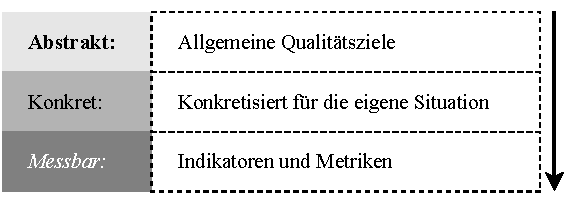
\includegraphics{contents/02_basics/res/quality_models.pdf}
    \caption{Aufbau eines Qualitätsmodells in drei Ebenen \cite[S. 34, ][]{schneider2012abenteuer}}
    \label{fig:basics_quality_models}
\end{figure}

Diese Arbeit entwickelt zwar kein Qualitätsmodell für \textit{Explainability}, enthält allerdings Zielvorschläge für die abstrakte Ebene des Modells. Im letzten Teil wird diese Basis verwendet, um Anforderungen für die Integration von Erklärungen in einem Beispielsystem aufzustellen. Welches Ziel diese Arbeit dabei verfolgt, wird im nächsten Kapitel vorgestellt.


% “Evaluating the quality of explanations is traditionally difficult due to their inherent subjectivity. The needs of different user groups can be very different, which is reflected in their expectations of what an explanation should offer.” \cite{martin_developing_2019, martin_evaluating_2021}

% Verschiedene SIGs z.B. \cite{do2010software}